\documentclass[12pt]{article}
\usepackage[a4paper]{geometry}
\usepackage[myheadings]{fullpage}
\usepackage{fancyhdr}
\usepackage{lastpage}
\usepackage{graphicx, wrapfig, subcaption, setspace, booktabs}
\usepackage[T1]{fontenc}
\usepackage[font=small, labelfont=bf]{caption}
\usepackage{fourier}
\usepackage[protrusion=true, expansion=true]{microtype}
\usepackage[english]{babel}
\usepackage{sectsty}
\usepackage{url, lipsum}
\usepackage{tgbonum}
\usepackage{hyperref}
\usepackage{xcolor}

\newcommand{\HRule}[1]{\rule{\linewidth}{#1}}
\onehalfspacing
\setcounter{tocdepth}{5}
\setcounter{secnumdepth}{5}


%%%%%%%%%%%%%%%%%%%%%%%%%%%%%%%%%%%%%%%%%%%%%%%%%%%%%%%%%%%%%%%%%%%%%%%%%%


\begin{document}
{\fontfamily{cmr}\selectfont
\title{ \normalsize \textsc{}
		\\ [2.0cm]
		\HRule{0.5pt} \\
		\LARGE \textbf{\uppercase{Proiect Proiectarea Algoritmilor Selecterea Activitatiilor}
		\HRule{2pt} \\ [0.5cm]
		\normalsize \today \vspace*{5\baselineskip}}
		}

\date{}

\author{
		Sotiraq Saraci \\ 
		Facultate de Automatica, Calculatoare si Tehnologia Informatiei  \\
		Calculatoare Romana, Anul I }

\maketitle
\newpage
\tableofcontents 

\vspace{70 mm} %70mm vertical space

\begin{abstract}
Acest  document  introduce  metodologia folosita de  realizare  a  temelor pentru cursul de Proiectarea algoritmilor.  Documentul contine,  de asemenea descrirea algoritmilor.
\end{abstract}
\newpage

%-------------------------------------------------------------------------------
% Section title formatting
\sectionfont{\scshape}
%-------------------------------------------------------------------------------

%-------------------------------------------------------------------------------
% BODY
%-------------------------------------------------------------------------------

\section{Introducere si Enuntul problemei}

Problemul se numește Selectare Activitațiilor. Este un problem faimos in campul de Proiectarea Algoritmilor mai specific in Greedy Algorithms. Enuntul problemei e asta: Se consideră o mulțime de activitați astfel încăt fiecare dintre ele necesită acces exclusiv la o resursă comună. Pentru fiecare activitate se cunoaște timpul de start și durata. Se cere determinarea unei submulțimi de cardinalitate maximă a acestor acivități de astfel încăt oricare două activități selectate sunt mutual compatibile (nu se suprapun în timp). Trebuie să implementam doi algoritmi diferiți.


\section{Algoritmi Propuși}

\begin{figure}[h]
\begin{center}
\begin{tabbing}
ACTIVITY-SELECTION($start, finish, number, i, j, k$) \\
1. \indent 			  \=$read$ $number$ \\
2. \indent            \> {\bf for}\= $k$ = $0$ to $number$ \\
3. \indent            \>			\>$read$ start[k] \\
4. \indent            \>			\>$read$ finish[k] \\
5. \indent            \> $read$ i, j \\
6. \indent            \>{\bf if} \=$start[j] >= finish[i]$ $and$ $start[j] >= finish[i]$ \\
7. \indent            \>            \>{\bf return} $1$ \\
8. \indent            \> {\bf else}  \\
10.\indent           \>				\>{\bf return} $0$ \\

\end{tabbing}
\caption{Algoritm de activitati selectate din utilizator.}
\label{fig_alg_ex}
\end{center}
\end{figure}
\begin{figure}[h]
\begin{center}
\begin{tabbing}
RANDOM-SELECTION($start, finish, number, i, j, temp$) \\
1. \indent 			  \=$read$ $number$ \\
2. \indent            \> {\bf for }\= $k$ = $0$ to $number$ \\
3. \indent            \>			\>$read$ start[k] \\
4. \indent            \>			\>$read$ finish[k] \\
5. \indent			  \>$temp$ = $0$\\
5. \indent			  \>{\bf while} \= $temp$ $not$ $equal$ $to$ $3$\\
5. \indent            \>			\>$i$ = $generateRandomInt$ ($0$, $number$)\\
5. \indent            \>			\>$j$ = $generateRandomInt$ ($0$, $number$)\\
5. \indent            \>			\>{\bf if} \=$i = j$\\
5. \indent            \>			\>				\>$temp++$\\
8. \indent            \>            \>{\bf else} \= $temp = 3$ \\
6. \indent            \>{\bf if} \=$start[j] >= finish[i]$ $and$ $start[j] >= finish[i]$ \\
7. \indent            \>            \>{\bf return} $1$ \\
8. \indent            \> {\bf else}  \\
10.\indent           \>				\>{\bf return} $0$ \\

\end{tabbing}
\caption{Algoritm de activitati selectate random.}
\label{fig_alg_ex}
\end{center}
\end{figure}
\vspace{20 mm} %70mm vertical space

\section{Datele experimentale}
Structura programului este simpla. Am creat un fisier "function.c" unde sunt sortat algoritmi si un fisier "main.c" unde programul este rulat. Am ales un interval de timp de 12 ori unde ia loc toate activitati. Este cerut din utilizator sa pune numar de activitatii si timpul de inceperea si terminarea. Testul meu contine 5 activitati cu timpuri ca mai jos:

\begin{center}
\begin{tabular}{| m{5em}|m{1cm}|m{1cm}|m{1cm}| m{1cm}|m{1cm} } 
\hline
Activity & A[0] & A[1] & A[2] & A[3] & A[4] \\ 
\hline
Start & 2 & 6 & 3 & 1 & 2 \\ 
\hline
Finish & 5 & 9 & 6 & 3 & 6 \\ 
\hline
\end{tabular}
\end{center}

\begin{figure}[htp]
    \centering
    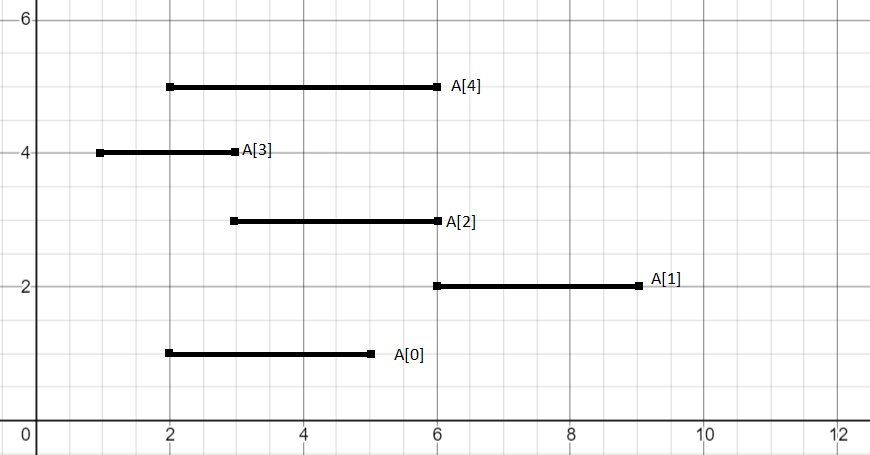
\includegraphics[width=10cm]{graph1.png}
    \caption{Activitati prezentate intr-un tabel}
    \label{fig:graph1}
\end{figure}


\section{Proiectarea experimentala a aplicației}
Dupa ce punem toate date de intrare, algoritmi o sa rulez. In primul algoritm algoritmul o sa compara doua date puse din utilizator. Dupa conditie daca timpul de start de activitatea[i] este mai mica sau egala cu timpul de terminare de activitatea[j] sau timpul de start de activitatea[j] este mai mare sau egala cu timpul de terminare de activitatea[i] algoritmul o sa ruleaza cu succes.

Acesta comparatie este valabil si pentru algoritmul 2, doar ca in algoritmul 2 numarul activitatii este selectat random. De asemena aici am pus o conditie ca permite executarea algoritmului nu mai putin decat 3 ori in cazul ca activitati selectate random sunt aceeasi. (De exemplu este ales activitate[3] and activitate[3].


\section{Rezultatele & concluziile} 
Dupa ce rulam programul nostru si am pus date de intrare primim rezultatele de mai jos:

\begin{figure}[htp]
    \centering
    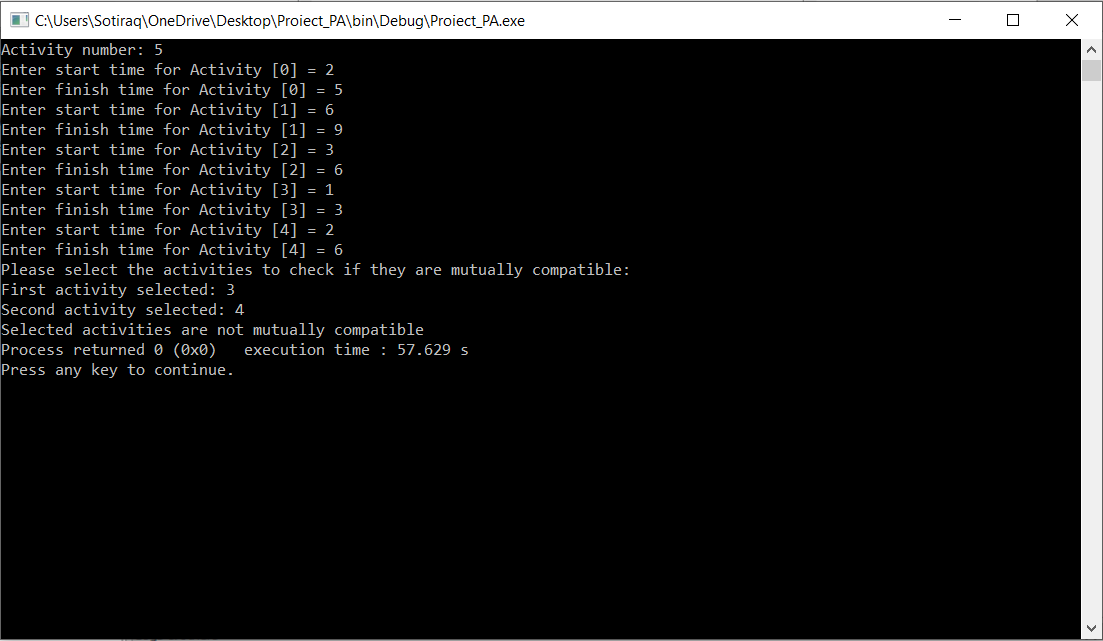
\includegraphics[width=10cm]{image1.png}
    \caption{Rularea de algoritmul 1}
    \label{fig:image1}
\end{figure}

\begin{figure}[htp]
    \centering
    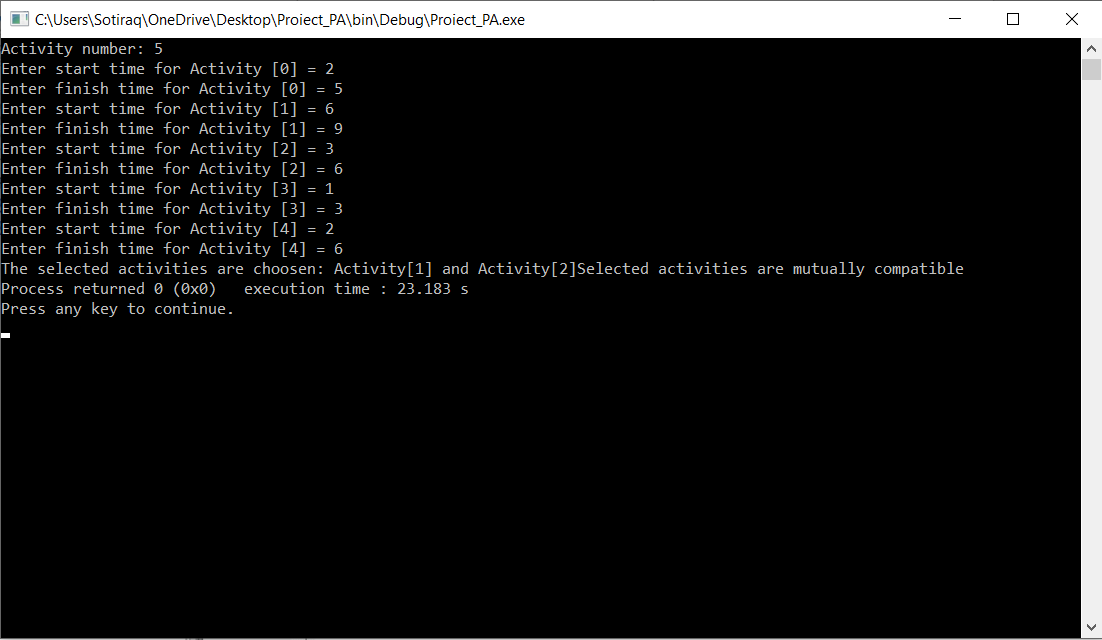
\includegraphics[width=10cm]{image2.png}
    \caption{Rularea de algoritmul 2}
    \label{fig:image2}
\end{figure}






\section{Referințile}


- www.euroinformatica.ro \\
- www.geeksforgeeks.org \\
- The C programing Language second edition - Ritchie and Kernighan



}
\end{document}


